\documentclass[11pt]{article}

\usepackage[margin=1.15in]{geometry}
\usepackage{amsmath}
\usepackage{amssymb}
\usepackage{graphicx}

% The reference layout, as the reader-facing text names it.
\newcommand{\dcom}{$\Delta d_{\rm com} = 62$~Mpc}
% The velocity dispersion of the Fingers-of-God blur.
\newcommand{\sv}{\sigma_v}
% An underscore after which a long code name may break.
\newcommand{\us}{\_\allowbreak}

% Floats sit near their first reference instead of drifting to
% figure-only pages.
\renewcommand{\topfraction}{0.9}
\renewcommand{\bottomfraction}{0.8}
\renewcommand{\textfraction}{0.07}
\renewcommand{\floatpagefraction}{0.85}
\setcounter{topnumber}{3}
\setcounter{totalnumber}{4}

\title{Cross spectra between thin redshift bins}
\date{November 2026}
\author{}

\begin{document}

\begin{center}
  {\LARGE Cross spectra between thin redshift bins\par}
  \vspace{0.6em}
  {\large Which pairs the data vector measures, and how the\\
    Fingers-of-God blur changes their overlap\par}
  \vspace{1em}
  {\large November 2026\par}
\end{center}
\vspace{1em}

\section{Summary}
\label{sec:summary}

\paragraph{The questions.}
The forecast cuts the DESI galaxies into thin redshift bins and
measures the angular power spectrum of every bin.  For some pairs of
bins it also measures their cross spectrum, the correlation between the
two bins' maps.  Four bin layouts slice the galaxies: \dcom{}, $76$ bins
of equal comoving depth, and three of fixed redshift width,
$\Delta z = 0.02$, $0.05$ and $0.2$, with $90$, $36$ and $10$ bins.  The
first two are the thin layouts.  This note answers three questions:
\begin{enumerate}
  \item How does the Fingers-of-God (FoG) blur, at its default
    strength, change how much neighbouring bins overlap?
  \item Which pairs of bins have their cross spectrum in the data
    vector, and why those?
  \item What does that rule mean in redshift, on each of the four bin
    layouts?
\end{enumerate}

\paragraph{The answers.}
\begin{enumerate}
  \item The blur has a width of $5$--$6$~Mpc along the line of sight,
    about a tenth of a thin bin.  It raises the overlap of two
    neighbouring thin bins from about $0.003$, the one grid step where
    their tabulated edges meet, to about $0.06$.  Bins one apart stay
    disjoint.  On \dcom{} the blur makes ten LRG3--ELG1 pairs overlap
    by $0.03$, half as much as a neighbour pair, although their raw
    ranges just miss; the data vector measures them too
    (Figure~\ref{fig:fog}).
  \item A pair is measured when the two bins' redshift distributions
    $n(z)$ overlap or touch, either as measured or once blurred by the
    FoG effect of item~1.  That gives the neighbours along each galaxy
    sample's chain of bins, plus the pairs of an LRG bin and an ELG bin
    at about the same redshift: at $0.8 < z < 1.1$ the LRG3 and ELG1
    groups are two galaxy samples observing one volume
    (Figures~\ref{fig:layouts} and~\ref{fig:zoom}).  The four layouts
    measure $107$, $133$, $52$ and $13$ cross spectra.
  \item On the layouts of fixed redshift width only adjacent bins pair.
    On \dcom{} the rule is adjacency in comoving distance, which no
    single cut in redshift can express: a bin of fixed comoving depth
    is $0.015$ wide in redshift at $z = 0.1$ and $0.035$ at $z = 1.5$.
\end{enumerate}

\paragraph{Beyond the current list.}
A further forecast measures what the pairs outside this rule would
add, along two axes: pairs whose raw ranges are up to three bin widths
apart, and pair lists selected with every dispersion raised to a
common test value (Section~\ref{sec:axes}).  On the three thinner
layouts those pairs raise the paper model's ${\rm FoM}(w_0, w_a)$ by
up to $55$--$59\%$, on $\Delta z = 0.2$ by at most $2\%$.  Attribution
fits trace the gain to the free level and slope of each sample
group's bias amplitude $\beta_i = b_{1,i}\,D(\bar{z}_i)$, the linear
bias times the growth factor: in the auto spectra the level is
degenerate with the clustering amplitude and the slope with the
evolution of growth that $w_0$ and $w_a$ control -- $\sv$ rides on
the same degeneracy -- while the cross spectra's correlation
coefficients do not depend on the linear bias, so the added pairs
separate the bias line from the growth history; with every nuisance
parameter held fixed they are worth only $2$--$8\%$
(Section~\ref{sec:bias}).  Every bias prior that passes the
project's accuracy test gives the same gain within a few percent;
under a prior on the bias levels and slopes themselves it would be
smaller, by an amount not yet computed, and whether any longer list
is adopted is the authors' choice.

\section{Fiducial model and parameter values}
\label{sec:fiducial}

Three of this note's figures (Figures~\ref{fig:fog},
\ref{fig:layouts} and~\ref{fig:zoom}) depend only on the shipped
redshift distributions, the pair lists and the default velocity
dispersions: no scale cut and no bias value enters them.  Only the
Fisher forecasts of Sections~\ref{sec:threshold} and~\ref{sec:axes}
run a fit.  This section freezes the values behind both, so the record
does not depend on configuration files that can change.

\paragraph{Geometry of the pair rule and the masks.}
The comoving distances of the \dcom{} slicing, of the pair rule and of
the shipped masks use $\chi(z)$ of a flat $\Lambda$CDM with
$H_0 = 67.32$~km/s/Mpc and $\Omega_m = 0.3$; the masks stop every bin
at $\ell + 1/2 \le k\,\chi(\bar{z}_i)$ with
$k = 0.1185\,{\rm Mpc}^{-1}$ (about $0.176\,h$/Mpc), with no growth
scaling.

\paragraph{Layouts and pairs.}
The four layouts hold $76$, $90$, $36$ and $10$ lens bins and measure
$107$, $133$, $52$ and $13$ cross pairs (\dcom{},
$\Delta z = 0.02$, $0.05$, $0.2$; Tables~\ref{tab:groups}
and~\ref{tab:counts}).  The paper data sets carry these pair lists;
the exploration examples keep the older $97$-pair \texttt{*\us linear}
files on \dcom{} (Section~\ref{sec:rule}).

\paragraph{Velocity dispersions.}
The fiducial dispersions are $371$, $358$, $357$, $348$, $343$, $304$
and $289$~km/s for the seven groups (BGS split at $\bar{z} = 0.255$),
with exploration prior widths $145$, $105$, $70$, $50$, $50$, $40$ and
$30$~km/s and paper widths six times these (Table~\ref{tab:sigv} and
Section~\ref{sec:fog}).  Every blur in this note runs at the
fiducials, except the pair selection on the $\sv$ axis of
Section~\ref{sec:axes}; the fit of Section~\ref{sec:threshold} uses
the exploration widths, the forecasts of Section~\ref{sec:axes} the
paper widths.

\paragraph{The pair-threshold fit.}
Its cosmology is the evaluate override of the example yamls:
$10^9 A_s = 2.1$ ($A_s$ the amplitude of the primordial curvature
power spectrum), $n_s = 0.96605$, $H_0 = 67.32$~km/s/Mpc,
$\Omega_b = 0.04$, $\Omega_m = 0.3$, $w_0 = -1$, $w_a = 0$,
$\sum m_\nu = 0.06$~eV and $\tau = 0.0697186$ fixed; the derived
$\sigma_8 = 0.8278$.  The linear bias is $b_{1,i} = B_g/D(\bar{z}_i)$
with $B_g = 1.34$ (BGS), $1.70$ (LRG1--LRG3) and $0.84$ (ELG1, ELG2),
under the pessimistic prior ($3\%$ correlated residuals, $L = 0.05$,
a free amplitude and tilt per group;
\texttt{notes/correlated\us bias\us prior\us v2}).  The higher-order
terms are model B + tilts (\texttt{notes/higher\us order\us bias}):
offsets $\Delta_2$ and $\Delta_s$ of widths $2$ and $1$, counterterms
$\alpha_0$ and $\alpha_2$ of width $0.5/k_{\rm max}^2$ at each cut,
stochastic amplitudes ${\rm SN}_0$ and ${\rm SN}_2$ of widths $2$ and
$5$, and flat tilts, with $\alpha_2$ free and the exploration $\sv$
widths: the reference model of
\texttt{notes/fog\us parameter\us degeneracy\us study}, not the paper
model, which fixes $\alpha_2 = 0$ in every bin and widens every $\sv$
prior sixfold.  The pair-axes forecasts of Section~\ref{sec:axes} run
the same cosmology and scale cut with the paper model.

\paragraph{Scale cut and covariance of the fit.}
The fit keeps the bands of the UV-fraction cut computed on the paper
model's fiducial at the final derivative tier
(\texttt{chains/model\us scale\us cuts\us final.npz}; a band is kept
while less than $5\%$ of it comes
from the power spectrum above $k_{\rm max}/D(\bar{z}_i)$),
intersected with the shipped mask.  The covariance is the Gaussian
covariance of the $107$-pair data set, built on the one-loop fiducial
($b_2$ and $b_{s^2}$ on their calibrations) with massless neutrinos
over $14{,}000$~deg$^2$, its inverse rescaled by $12{,}300/14{,}000$.
The forecasts of Section~\ref{sec:axes} build the same Gaussian
covariance on each layout's largest pair list.

\section{Why cross spectra between thin bins matter}
\label{sec:why}

\paragraph{The angular power spectrum.}
Take the galaxies of bin $i$ and draw a map of their number on the
sky: $\delta_i(\hat{n})$ is the fractional excess of galaxies in the
direction $\hat{n}$ over the mean.  Expand the map in spherical
harmonics, $\delta_i(\hat{n}) = \sum_{\ell m} a^i_{\ell m}
Y_{\ell m}(\hat{n})$.  The multipole $\ell$ labels an angular scale of
about $180^\circ/\ell$: $\ell = 20$ is about $9^\circ$, $\ell = 500$
about $0.4^\circ$.

The auto spectrum of bin $i$ is the variance of its coefficients,
$C^{ii}_\ell = \langle |a^i_{\ell m}|^2 \rangle$; the cross spectrum of
bins $i$ and $j$ is their covariance, $C^{ij}_\ell = \langle a^i_{\ell
m} a^{j*}_{\ell m} \rangle$.  Two unrelated maps have a cross spectrum
that averages to zero; two maps of the same structures have a positive
one.  The data vector holds these spectra in $53$ bands of width
$\Delta\ell = 10$ over $15 \le \ell \le 544$.

\paragraph{Why neighbouring thin bins correlate.}
A thin bin is a shell of the universe a few tens of Mpc deep: $62$~Mpc
on \dcom{}, and between $37$ and $85$~Mpc for $\Delta z = 0.02$.  The
matter distribution has structures of every size.  One that is
$200$~Mpc across spans three or four such shells, and each of them sees
it in the same direction on the sky.  Their maps share it, so the cross
spectrum of two neighbouring shells is large at the angular scale of
that structure.  A structure a few Mpc across sits in one shell only,
unless it sits where two shells meet.

\paragraph{Limber and non-Limber.}
These two cases are the two regimes of a cross spectrum.  At high
$\ell$ the Limber approximation~\cite{Limber1953} holds: only Fourier
modes perpendicular to the line of sight contribute, and
\begin{equation}
  C^{ij}_\ell \;\simeq\; \int d\chi\, \frac{W_i(\chi)\,W_j(\chi)}{\chi^2}\,
  P\!\left(k = \frac{\ell + 1/2}{\chi}\right) ,
  \label{eq:limber}
\end{equation}
with $\chi$ the comoving distance, $W_i(\chi)$ the redshift
distribution of bin $i$ written per unit comoving distance, and $P(k)$
the power spectrum of the galaxy density at wavenumber $k$.  Two shells
whose $W$ do not overlap then have no cross spectrum.  At low $\ell$
the approximation fails for thin shells: modes with a component along
the line of sight longer than the shell depth connect shells that do
not touch.  The forecast computes every spectrum without the Limber
approximation, so it keeps that low-$\ell$ correlation.

\paragraph{Where the radial information sits.}
Slicing a sample into thin shells keeps information along the line of
sight: a shell of depth $\Delta\chi$ resolves line-of-sight wavenumbers
up to about $\pi/\Delta\chi$, $0.05\,{\rm Mpc}^{-1}$ for $62$~Mpc.  The
auto spectra say how clustered each shell is; the cross spectra say how
the clustering of one shell continues into the next.

How much the cross spectra are worth depends on the bin layout:
the thinner the shells, the more of the line-of-sight information
sits in the cross spectra between neighbours rather than in the
auto spectra.

\section{The six groups and the LRG--ELG overlap}
\label{sec:groups}

\paragraph{Three galaxy samples.}
DESI selects three kinds of galaxies, each by its own colours and
brightness, and each fills the redshifts where it is bright and
numerous enough to observe:
\begin{itemize}
  \item \textbf{BGS}, the Bright Galaxy Survey: the brightest galaxies
    at low redshift, here $0.1 < z < 0.4$;
  \item \textbf{LRG}, luminous red galaxies: massive galaxies that
    stopped forming stars, $0.4 < z < 1.1$;
  \item \textbf{ELG}, emission-line galaxies: star-forming galaxies,
    found by the bright emission lines of their gas, $0.8 < z < 1.6$.
\end{itemize}
Nothing forces these ranges to tile the redshift axis.  LRG and ELG
both cover $0.8 < z < 1.1$.

\paragraph{Six groups.}
The forecast splits the samples into six groups by the bins' mean
redshift $\bar{z}_i$, and gives each group its own bias parameters
(Table~\ref{tab:groups}): BGS whole; LRG1 ($\bar{z}_i < 0.6$), LRG2
($0.6 \le \bar{z}_i < 0.8$) and LRG3 ($\bar{z}_i \ge 0.8$); ELG1
($\bar{z}_i < 1.1$) and ELG2 ($\bar{z}_i \ge 1.1$).  LRG3 and ELG1 are
therefore two different galaxy populations in the same volume, at
$z \approx 0.8$--$1.1$.

\begin{table}[ht]
  \centering
  \begin{tabular}{llcc}
    \hline
    group & sample & bins & $\bar{z}_i$ \\
    \hline
    BGS & bright galaxies & $1$--$18$ & $0.11$--$0.38$ \\
    LRG1 & luminous red galaxies & $19$--$29$ & $0.41$--$0.60$ \\
    LRG2 & luminous red galaxies & $30$--$38$ & $0.62$--$0.79$ \\
    LRG3 & luminous red galaxies & $39$--$49$ & $0.81$--$1.06$ \\
    ELG1 & emission-line galaxies & $50$--$61$ & $0.81$--$1.09$ \\
    ELG2 & emission-line galaxies & $62$--$76$ & $1.11$--$1.55$ \\
    \hline
  \end{tabular}
  \caption{The six groups of \dcom{}, with bins numbered from $1$ in
    data-vector order.  LRG3 and ELG1 cover the same redshifts.}
  \label{tab:groups}
\end{table}

\paragraph{The numbering runs group by group.}
Bins are numbered in the order of the data vector: all BGS bins by
increasing redshift, then all LRG bins, then all ELG bins.  The
numbering therefore jumps back in redshift between bins $49$ and $50$:
bin $49$ (LRG3) has $\bar{z} = 1.060$, bin $50$ (ELG1) has
$\bar{z} = 0.812$.  Two bins far apart in number can sit at the same
redshift: LRG3 bin $44$ has $\bar{z} = 0.932$ and ELG1 bin $55$ has
$\bar{z} = 0.931$.

\paragraph{What the LRG--ELG cross spectrum measures.}
An LRG bin and an ELG bin at the same redshift sample the same matter
with different galaxies.  On large scales a galaxy map is the matter map
times a number, the linear bias $b_i$ of the bin, so their cross
spectrum is about $b_i b_j$ times the matter spectrum, while the two
autos are about $b_i^2$ and $b_j^2$ times it.  The three spectra
together tie the two biases to each other.  Two tracers of the same
structures also share the random fluctuations of those structures, so
comparing them measures their bias ratio with less of that randomness
than either map alone (the multi-tracer idea~\cite{Seljak2009}).

\paragraph{Shot noise and the stochastic terms.}
A galaxy map is made of discrete objects, so even a random scatter of
galaxies has a nonzero auto spectrum: the shot noise, $1/\bar{n}_i$
for a bin of $\bar{n}_i$ galaxies per steradian.  A cross spectrum
has no shot noise, because no galaxy is in two bins: within one
sample each galaxy has one measured redshift, and two samples are
different galaxies.

The one-loop model adds stochastic terms beyond this Poisson noise,
${\rm SN}_0$ and ${\rm SN}_2$.  They are properties of the
three-dimensional galaxy field, so they reach the cross spectrum of two
bins of one sample through the overlap of their kernels, $\int d\chi\,
W_i W_j/\chi^2$ for ${\rm SN}_0$ and the same integral of the kernels'
radial derivatives for ${\rm SN}_2$ (\texttt{stochastic\us templates} in
\texttt{likelihood/desi\us cl.py}).  An LRG--ELG pair gets none: two
different populations do not share a stochastic term, and the model has
no separate cross-stochasticity parameter.

\section{The Fingers-of-God blur}
\label{sec:fog}

\subsection{What it is}

\paragraph{Redshift is not distance.}
The forecast places each galaxy by its measured redshift.  That
redshift has two parts: the cosmological redshift, set by the
galaxy's distance, and a Doppler shift from the galaxy's own velocity
$v$ along the line of sight, its peculiar velocity.  The two multiply,
$1 + z_{\rm obs} = (1 + z)(1 + v/c)$, so for $v \ll c$
\begin{equation}
  z_{\rm obs} - z \;\simeq\; (1 + z)\,\frac{v}{c} .
  \label{eq:doppler}
\end{equation}
For example, $v = 350$~km/s at $z = 0.5$ shifts the redshift by
$1.75 \times 10^{-3}$.  In distance this is $\delta\chi = c\,\delta
z/H(z) = (1 + z)\,v/H(z) \approx 6$~Mpc, with $H(0.5) = 88$~km/s/Mpc
in the examples' cosmology ($H_0 = 67.32$~km/s/Mpc, $\Omega_m = 0.3$).

\paragraph{Fingers of God.}
Inside groups and clusters, galaxies orbit their common halo with
random speeds of several hundred km/s.  In a map that places every
galaxy at its redshift distance, a cluster is stretched along the line
of sight into a long finger pointing at the observer: the Fingers of
God~\cite{Jackson1972}.  The orderly infall of galaxies onto large
structures is a different effect, the Kaiser
distortion~\cite{Kaiser1987}, which the model computes separately.

\paragraph{What it does to a thin bin.}
A bin collects the galaxies whose measured redshift falls inside its
range: a sharp cut in $z_{\rm obs}$.  The matter that the galaxies
trace sits at their true distances.  A galaxy just outside the range,
moving towards it, is measured inside; one just inside, moving away, is
measured outside.  So the galaxies of the bin trace the matter over a
slightly wider, softer-edged range than the histogram of their measured
redshifts.  The same convolution describes a sharp shell in true
redshift observed blurred along the line of sight; for a symmetric
velocity distribution the two descriptions agree.

\subsection{The model in the likelihood}

The likelihood replaces each bin's raw $n_i(z)$ by its convolution with
a Gaussian in redshift~\cite{GrasshornGebhardt2020},
\begin{equation}
  n_i^{\rm FoG}(z) = \int dz'\, n_i(z')\,
  \frac{1}{\sqrt{2\pi}\,\sigma_{z,i}}\,
  \exp\!\left[-\frac{(z - z')^2}{2\sigma_{z,i}^2}\right] ,
  \qquad
  \sigma_{z,i} = (1 + \bar{z}_i)\,\frac{\sv}{c} ,
  \label{eq:fog}
\end{equation}
with $\sv$ the velocity dispersion of the bin's group, the standard
deviation of the line-of-sight velocities, and $c = 299792.458$~km/s.
The width follows from Eq.~\eqref{eq:doppler}.

The code is \texttt{set\us lens\us related} in
\texttt{likelihood/desi\us cl.py}.  It convolves a copy of each raw
histogram with \texttt{scipy.ndimage.gaussian\us filter1d} on the
$n(z)$ table's grid, the DESI grid refined five-fold (step
$7.0 \times 10^{-5}$, so $\sigma_{z,i}$ spans $20$ to $36$ steps), with
the width in grid steps and zero beyond the grid ends.  The Gaussian is
truncated at $4\sigma_{z,i}$, scipy's default.  The $\sv$ are sampled
parameters, so the convolution runs again at every sampled point.  The
figures of this note repeat that call; at the default $\sv$ the result
equals, bit for bit, the convolved tables that the covariance adapter
writes with the same call (\texttt{covariance/<layout>\us fog.nz}).

\subsection{Where the velocity dispersions come from}

The source forecast measured the line-of-sight velocity dispersion of
its simulated galaxies as a function of redshift, with an error bar per
bin.  The project reads one value per group off that measurement
(Table~\ref{tab:sigv}).  The measured curve steps inside BGS, between
the bins at $\bar{z} = 0.247$ and $0.263$, so BGS takes two values,
split at $z = 0.255$: seven dispersion groups for six bias groups.

\begin{table}[ht]
  \centering
  \begin{tabular}{lccccc}
    \hline
    group & $\sv$ [km/s] & exploration width & paper width
      & $\sigma_{z,i}$ [$10^{-3}$] & $\delta\chi$ [Mpc] \\
    \hline
    BGS, $\bar{z}_i < 0.255$ & $371$ & $145$ & $870$ & $1.37$--$1.54$ & $5.8$--$6.1$ \\
    BGS, $\bar{z}_i \ge 0.255$ & $358$ & $105$ & $630$ & $1.51$--$1.65$ & $5.9$--$6.0$ \\
    LRG1 & $357$ & $70$ & $420$ & $1.68$--$1.90$ & $6.0$--$6.1$ \\
    LRG2 & $348$ & $50$ & $300$ & $1.88$--$2.08$ & $6.0$ \\
    LRG3 & $343$ & $50$ & $300$ & $2.07$--$2.36$ & $5.8$--$5.9$ \\
    ELG1 & $304$ & $40$ & $240$ & $1.84$--$2.12$ & $5.1$--$5.2$ \\
    ELG2 & $289$ & $30$ & $180$ & $2.04$--$2.46$ & $4.6$--$4.8$ \\
    \hline
  \end{tabular}
  \caption{The default velocity dispersion of each group, the widths of
    its Gaussian prior in the exploration files and in the paper model
    (six times the exploration width; both in km/s), and the resulting
    redshift width $\sigma_{z,i}$ and comoving width
    $\delta\chi = (1 + \bar{z}_i)\,\sv/H(\bar{z}_i)$ over the bins of
    \dcom{}.}
  \label{tab:sigv}
\end{table}

Each prior is a Gaussian centred on the default and truncated at zero.
The exploration width is five times the per-bin error bar of the
measurement; the paper model multiplies every width by six, so that
the sampled dispersions can absorb the radial counterterm it drops
(\texttt{notes/fog\us parameter\us degeneracy\us study}).  At the
sixfold width the truncation matters for the first BGS group: it
removes $33\%$ of the Gaussian, and the truncated mean is about
$850$~km/s, while the Fisher forecasts treat every $\sv$ prior as an
untruncated Gaussian about the default.  The exploration defaults and
widths live in \texttt{likelihood/params\us desi*.yaml} (the
\texttt{DESI\us SIGV} parameters; the first bin of each group carries
the prior and the others are tied to it), the paper widths in
\texttt{likelihood/params\us desi*\us bias\us pessimistic.yaml}, and
the same seven defaults in \texttt{CHUNK\us SIGMA\us V} of
\texttt{covariance/lssty1xdesi\us covariance.py}, which convolves the
covariance's kernels at fixed $\sv$.  Every figure of this note blurs
at the defaults, except that the $\sv$ axis of Section~\ref{sec:axes}
selects pairs with the blur at a common test dispersion; the fit of
Section~\ref{sec:threshold} uses the exploration widths
(Section~\ref{sec:fiducial}).  The ELG dispersions
are the lowest, as expected for star-forming galaxies, which tend to
live in lighter halos with slower orbits.

\subsection{How large the blur is}

\paragraph{A nearly constant width in distance.}
In comoving distance the blur is $\delta\chi = (1 + z)\,\sv/H(z)$
(last column of Table~\ref{tab:sigv}): $5.8$--$6.1$~Mpc for BGS and
LRG and $4.6$--$5.2$~Mpc for ELG, at every redshift.  It barely changes
with $z$ because $(1 + z)/H(z)$ changes by at most $10\%$ over
$0.1 < z < 1.6$.

\paragraph{Against the bin width.}
What matters for overlap is $\sigma_{z,i}$ divided by the bin's width
$w_i$, the redshift range its galaxies were selected in.  On \dcom{} it
is the same ratio in distance, $\delta\chi/62$~Mpc: $0.069$--$0.096$,
about a tenth of the bin at every redshift.  On $\Delta z = 0.02$ it
grows with redshift, from $0.069$ to $0.125$, because a fixed
$\Delta z$ is a thinner shell at high $z$.  On $\Delta z = 0.05$ it is
$0.028$--$0.050$, and on $\Delta z = 0.2$ $0.007$--$0.023$
(Figure~\ref{fig:fog}, top right).

A Gaussian blur of a sharp edge moves a fraction of about
$\sigma_z/(\sqrt{2\pi}\,w)$ of a bin's galaxies across each edge.  The
blurred $n(z)$ of a thin bin has $5$--$8\%$ of its weight outside its
raw range on \dcom{} and $5$--$10\%$ on $\Delta z = 0.02$, against
$2$--$4\%$ on $\Delta z = 0.05$ and $0.5$--$2\%$ on $\Delta z = 0.2$.
That weight lies inside the neighbouring bins.

\subsection{What it does to the overlap}
\label{sec:overlap}

\paragraph{A measure of overlap.}
For two bins define the normalized overlap integral
\begin{equation}
  O_{ij} \;=\; \frac{\int dz\, n_i(z)\, n_j(z)}
  {\sqrt{\int dz\, n_i^2(z)\, \int dz\, n_j^2(z)}} ,
  \label{eq:overlap}
\end{equation}
$1$ for two identical distributions and $0$ for disjoint ones,
whatever their normalization.  It has a direct meaning.  In the Limber
regime, Eq.~\eqref{eq:limber}, the power spectrum and $\chi$ barely
change across two thin bins, so $O_{ij}$ is close to the correlation
coefficient $C^{ij}_\ell/\sqrt{C^{ii}_\ell C^{jj}_\ell}$ of the two
bins at high $\ell$.  The ${\rm SN}_0$ cross term of
Section~\ref{sec:groups} is nearly the same integral.

\paragraph{Neighbours.}
Without the blur, two neighbouring bins touch only over the one grid
step where their tabulated edges meet, and their overlap is about
$h/(6\,w)$: $0.0015$--$0.0039$ on \dcom{}, $0.0027$--$0.0029$ on
$\Delta z = 0.02$, $0.0011$--$0.0012$ on $\Delta z = 0.05$ and
$0.0003$--$0.0004$ on $\Delta z = 0.2$.  This number measures the grid,
not the galaxies.  With the blur at the default $\sv$ the edges become
ramps about $4\sigma_z$ wide, and the overlap becomes about
$0.6\,\sigma_z/w$: $0.039$--$0.061$ on \dcom{} (median $0.057$),
$0.043$--$0.083$ on $\Delta z = 0.02$ ($0.066$), $0.018$--$0.032$ on
$\Delta z = 0.05$ ($0.024$) and $0.006$--$0.009$ on $\Delta z = 0.2$
($0.007$).  On the thin layouts this is a $6\%$ correlation at high
$\ell$ that the raw $n(z)$ would put at $0.3\%$.

\paragraph{Bins one apart stay disjoint.}
The bin between them is at least $8\sigma_z$ wide, and the Gaussian is
truncated at $4\sigma_z$, so the blurred $n(z)$ of two bins one apart
do not meet.  The only exception is the last ELG2 bins of
$\Delta z = 0.02$, where $\sigma_z/w = 0.125$ and the truncated tails
touch, with an overlap below $2 \times 10^{-14}$.  Even an untruncated
Gaussian gives two blurred top hats one bin apart a percent-level
overlap only at $\sigma_z \approx 0.4\,w$, four times the default on the
thin layouts.  Within two prior widths of every default $\sigma_z/w$
stays below $0.2$, where that overlap is below $2 \times 10^{-5}$.

\begin{figure}[t]
  \centering
  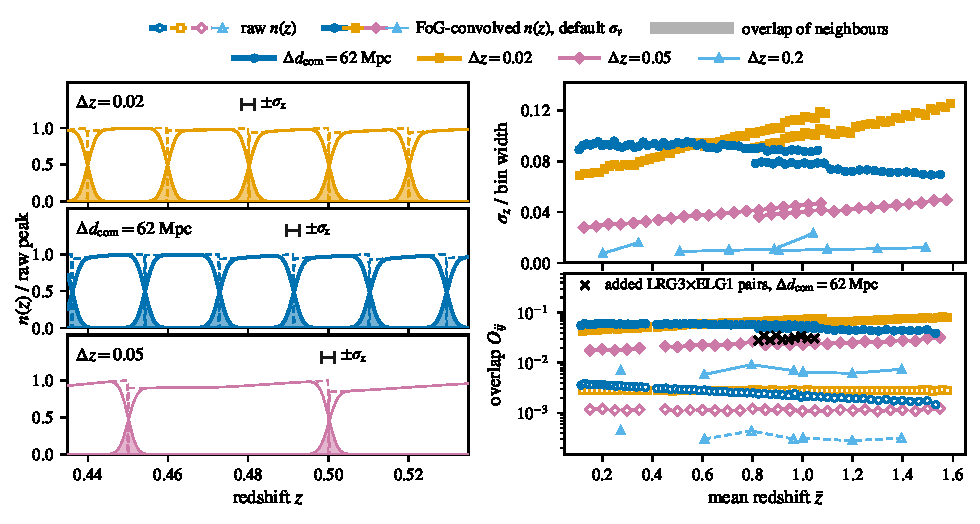
\includegraphics[width=\linewidth]{plots/fog_smearing/fog_smearing.pdf}
  \caption{The Fingers-of-God blur at the default $\sv$.  Left: raw
    (dashed) and blurred (solid) $n(z)$ of the LRG1 bins in
    $0.435 < z < 0.535$ on three layouts, each divided by its raw
    peak; shaded: the overlap $\min(n_i, n_j)$ of neighbouring blurred
    bins; bar: $\pm\sigma_z$.  Right: $\sigma_z$ over the bin width,
    and the overlap $O_{ij}$ of Eq.~\eqref{eq:overlap} for
    consecutive bins of one sample, raw (dashed, open markers) and
    blurred (solid, filled), against the mean redshift.  Crosses: the
    ten LRG3--ELG1 pairs of \dcom{} that the second step of the pair
    rule (Section~\ref{sec:rule}) adds, whose raw overlap is zero.  Bins one apart overlap by at most $2 \times 10^{-14}$, raw
    or blurred.}
  \label{fig:fog}
\end{figure}

\section{Which pairs are measured}
\label{sec:rule}

\paragraph{The first step: raw ranges.}
Each bin's raw $n(z)$ is the histogram of the measured redshifts of its
galaxies, tabulated on the DESI redshift grid of step
$h = 3.5 \times 10^{-4}$.  Let $z_i^{\rm lo}$ and $z_i^{\rm hi}$ be the
first and last grid redshifts where $n_i(z)$ is nonzero.  Bins $i$ and
$j$ pair when their ranges overlap or touch:
\begin{equation}
  z_j^{\rm lo} \le z_i^{\rm hi} + 1.5\,h
  \quad\text{and}\quad
  z_i^{\rm lo} \le z_j^{\rm hi} + 1.5\,h .
  \label{eq:rule}
\end{equation}
The slack of $1.5$ grid steps is there because two neighbouring bins of
one sample either share their edge node or sit one node apart; $1.5$
steps catches both and nothing farther.

For example, on $\Delta z = 0.02$ bin $1$ ends at $z = 0.1198$ and bin
$2$ starts one grid step later, at $0.1202$: they pair.  Bin $3$ starts
at $0.1401$, $0.020$ after the end of bin $1$: bins $1$ and $3$ do not
pair.

\paragraph{The second step: blurred kernels.}
The model never uses the raw $n(z)$ directly.  It first blurs each one
by the Fingers-of-God effect of Section~\ref{sec:fog}, which spreads
every bin a few Mpc beyond its edges.  Two bins whose raw ranges just
miss can therefore still overlap once blurred.  The second step adds
every such pair: bins $i$ and $j$ also pair when their blurred $n(z)$
overlap at all, $O_{ij} \ge 10^{-6}$ at the default velocity
dispersions, with $O_{ij}$ the normalized overlap integral of
Eq.~\eqref{eq:overlap} (\texttt{scripts/make\us desi\us pairs.py}).

The threshold is not a tuning.  Before this step the blurred overlaps
of unmeasured pairs fall into two sets far apart: ten pairs at
$0.028$--$0.035$, and every other pair below $2 \times 10^{-14}$, the
reach of the truncated Gaussian tails.  Any threshold between $10^{-6}$
and $0.0277$ gives the same lists: those ten pairs on \dcom{}, none on
the fixed-$\Delta z$ layouts.

\paragraph{Where the pair lists come from.}
For the three fixed-$\Delta z$ layouts the first step writes the pair
list (\texttt{cross\us pairs} in \texttt{scripts/make\us desi\us
dz\us case.py}), and the second adds nothing.  On \dcom{} the first
list comes from the DESI forecast's data file (a \texttt{sacc} file),
which pairs bins by redshift proximity; \texttt{scripts/make\us
desi\us dataset.py} imports it.  The first step reproduces $96$ of its
$97$ pairs.  The exception is the boundary pair of BGS bin $18$ and
LRG1 bin $19$: BGS ends at $z = 0.390$ and LRG starts at $z = 0.400$,
so their ranges are $0.010$ apart, and the forecast includes them
anyway; the list keeps it.  Blurred, their kernels overlap by only
$3 \times 10^{-7}$: the ranges are six times $\sigma_z$ apart.  The second step adds ten LRG3--ELG1 pairs
(Section~\ref{sec:redshift}), for $107$ pairs in all.

\paragraph{The \dcom{} data vector.}
With the added pairs the \dcom{} data vector holds $198$ spectra:
$15$ cosmic-shear spectra, $76$ autos and $107$ cross spectra, in $53$
bands each, $10{,}494$ entries of which the mask keeps $5{,}674$.  Each
added pair keeps the bands where both of its autos are kept, the rule
every other pair follows.  The Gaussian covariance rebuilt on this
layout is positive definite and bitwise equal to the $97$-pair
covariance on the shared spectra.  The exploration examples keep the $97$-pair files
(the \texttt{*\us linear} dataset, mask, pair list and covariance), so
their $\chi^2$ values stay as committed.

\paragraph{The counts.}
Table~\ref{tab:counts} sorts every layout's pairs by kind.  Most join a
bin to the next one of its sample.  The rest join an LRG and an ELG bin:
the LRG3--ELG1 pairs of the shared volume (on \dcom{}, $22$ from the
first step and $10$ from the second), one LRG2--ELG1 pair at $z = 0.8$
where LRG2 ends and ELG1 begins, and, on $\Delta z = 0.02$ and $0.05$,
one LRG3--ELG2 pair at $z = 1.1$.  Each bin has $1$ to $5$ cross
partners, $1$ to $4$ on $\Delta z = 0.2$; the first and last bins have
one.

\begin{table}[ht]
  \centering
  \small
  \setlength{\tabcolsep}{4.5pt}
  \begin{tabular}{lccccccc}
    \hline
    layout & bins & next bin & BGS--LRG1 & LRG3--ELG1 & LRG--ELG, other
      & added & total \\
    \hline
    \dcom{} & $76$ & $73$ & $1$ & $22$ & $1$ & $10$ & $107$ \\
    $\Delta z = 0.02$ & $90$ & $87$ & $1$ & $43$ & $2$ & $0$ & $133$ \\
    $\Delta z = 0.05$ & $36$ & $33$ & $1$ & $16$ & $2$ & $0$ & $52$ \\
    $\Delta z = 0.2$ & $10$ & $7$ & $1$ & $4$ & $1$ & $0$ & $13$ \\
    \hline
  \end{tabular}
  \caption{The measured cross spectra of each layout, by kind.
    ``Next bin'': two consecutive bins of one sample; BGS--LRG1: the
    pair across the BGS--LRG boundary at $z = 0.4$; ``LRG--ELG,
    other'': the LRG2--ELG1 pair at $z = 0.8$ and the LRG3--ELG2 pair at
    $z = 1.1$; ``added'': the LRG3--ELG1 pairs of the second step, whose
    raw ranges miss and whose blurred $n(z)$ overlap.}
  \label{tab:counts}
\end{table}

\paragraph{How to read Figure~\ref{fig:layouts}.}
Each block is one layout.  Its upper panel draws every bin's raw
$n(z)$ at unit peak, BGS and LRG in the upper lane, ELG in the lower
one; two bins that touch share an edge.  Its lower panel is the pair
graph: a dot per bin at $\bar{z}_i$ and a segment per measured pair.
The segments inside a row are the chain of neighbours; the segments
between the rows are the LRG--ELG pairs, all inside the gray band
where LRG3 and ELG1 share a volume, or at its edges.  The
dash-dotted vermillion segments of \dcom{} are the ten pairs of the
second step.  On $\Delta z = 0.02$ the LRG and ELG bins have the same
edges, so each
LRG3 bin touches three ELG1 bins: the one at its redshift and the two
beside it.  Figure~\ref{fig:zoom} magnifies the corner where LRG2 ends
and LRG3 and ELG1 begin.

\begin{figure}[tbp]
  \centering
  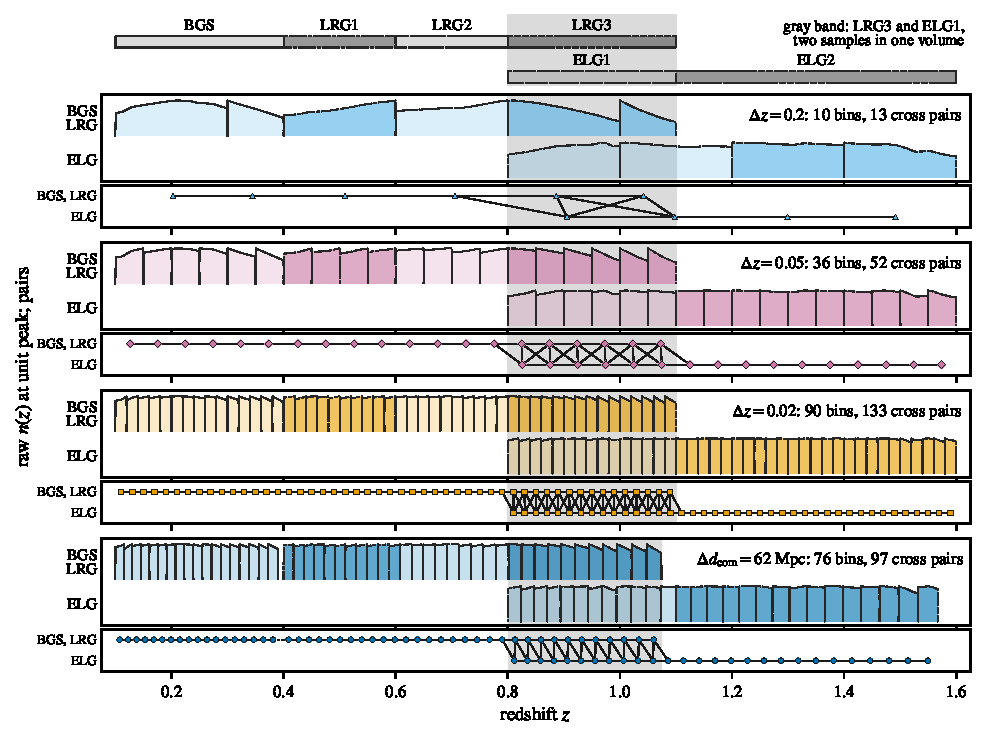
\includegraphics[width=\linewidth]{plots/nz_overlap_layouts/nz_overlap_layouts.pdf}
  \caption{Every thin bin of the four layouts and the cross spectra the
    data vector measures.  Upper panel of each block: each bin's raw
    $n(z)$ at unit peak, BGS and LRG in the upper lane, ELG in the
    lower; fill shade and outline style mark the six groups (header).
    Lower panel: a dot per bin at its mean redshift and a segment per
    measured pair; solid: raw ranges overlap or touch; dashed: the
    BGS--LRG1 pair of \dcom{}, whose ranges do not touch; dash-dotted
    vermillion: the ten LRG3--ELG1 pairs added because their blurred
    $n(z)$ overlap.  Gray band: the redshifts where LRG3 and ELG1 both
    have bins.}
  \label{fig:layouts}
\end{figure}

\begin{figure}[t]
  \centering
  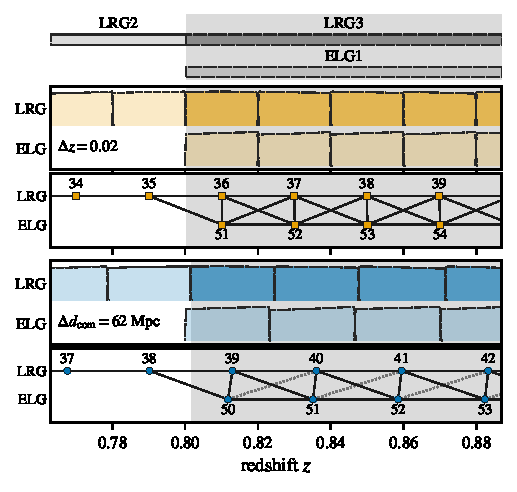
\includegraphics[width=3.5in]{plots/nz_overlap_zoom/nz_overlap_zoom.pdf}
  \caption{The corner of Figure~\ref{fig:layouts} where LRG2 ends and
    LRG3 and ELG1 begin, on the two thin layouts, with every bin
    numbered in data-vector order.  Solid: measured pairs whose raw
    ranges overlap or touch.  Dash-dotted vermillion: the LRG3--ELG1
    pairs of \dcom{} whose raw ranges miss by $3$ to $5$ grid steps and
    which the second step adds because their blurred $n(z)$ overlap
    (Section~\ref{sec:fog}).  A segment leaving the panel joins a bin
    outside it.}
  \label{fig:zoom}
\end{figure}

\section{What the rule means in redshift}
\label{sec:redshift}

\paragraph{Centre separations.}
A rule in terms of ranges can be compared with a rule in terms of
centres: is there a separation $|\bar{z}_i - \bar{z}_j|$ below which
every pair is measured and above which none is?
Table~\ref{tab:separations} gives, per layout, the largest separation
of a measured pair and the smallest of an unmeasured one.

\begin{table}[ht]
  \centering
  \small
  \begin{tabular}{lccc}
    \hline
    layout & bin width in $z$ & largest measured & smallest unmeasured \\
    \hline
    $\Delta z = 0.2$ & $0.1$--$0.2$ & $0.211$ (LRG3 $5$, ELG1 $8$)
      & $0.257$ (LRG3 $6$, ELG2 $9$) \\
    $\Delta z = 0.05$ & $0.05$ & $0.053$ (BGS $6$, LRG1 $7$)
      & $0.097$ (LRG3 $18$, ELG1 $22$) \\
    $\Delta z = 0.02$ & $0.02$ & $0.020$ (LRG3 $48$, ELG1 $64$)
      & $0.040$ (LRG3 $45$, ELG1 $58$) \\
    \dcom{} & $0.015$--$0.035$ & $0.035$ (ELG2 $75$, $76$)
      & $0.030$ (BGS $1$, $3$) \\
    \hline
  \end{tabular}
  \caption{The separation $|\bar{z}_i - \bar{z}_j|$ of the mean
    redshifts of the farthest measured pair and of the closest
    unmeasured pair, with their groups and bin numbers.  On
    $\Delta z = 0.2$ the bins at the ends of some samples are $0.1$
    wide.}
  \label{tab:separations}
\end{table}

\paragraph{Fixed redshift width: only adjacent bins.}
On the three fixed-$\Delta z$ layouts the two columns are separated by
about a factor of two: neighbours are one width apart, the next bin
over is two widths apart.  Any cut between the two columns, for
example at $0.03$ on $\Delta z = 0.02$, reproduces the rule.  So on
these layouts the rule means: only adjacent bins pair,
where an LRG bin and an ELG bin with the same range count as adjacent
(separation near zero).  The edge bins of $\Delta z = 0.2$, $0.1$
wide, shift the numbers but not the conclusion.

\paragraph{Fixed comoving width: no redshift cut works.}
On \dcom{} the columns cross: a measured pair is $0.035$ apart and an
unmeasured one $0.030$.  The reason is how a shell of fixed depth
looks in redshift.  The comoving distance is $\chi(z) = \int_0^z c\,
dz'/H(z')$, with $H(z)$ the expansion rate, so a shell of depth
$\Delta d_{\rm com}$ spans $\Delta z \approx \Delta d_{\rm com}\,
H(z)/c$ in redshift.  $H$ grows with $z$, so the same $62$~Mpc covers
$0.015$ in redshift at $\bar{z} = 0.11$ and $0.035$ at
$\bar{z} = 1.55$.

Two examples make this concrete.  BGS bins $1$ and $3$, one bin apart
at $z \approx 0.12$, are only $0.030$ apart in mean redshift and not
paired; ELG2 bins $75$ and $76$, neighbours at $z \approx 1.53$, are
$0.035$ apart and paired.  The rule is adjacency in comoving distance,
and in redshift that adjacency stretches with $z$.

\paragraph{Misaligned LRG and ELG edges.}
The LRG3--ELG1 pairs of \dcom{} show a second effect.  Each sample has
its own bin edges: the LRG
bins begin at $z = 0.400$ and the ELG bins at $z = 0.800$.  In the
shared volume the LRG edges sit $0.001$--$0.002$ above the ELG edges
(Figure~\ref{fig:zoom}, bottom).  An LRG3 bin therefore
overlaps the ELG1 bin at its redshift and the one above it, and starts
just above the end of the one below it.  Bin $40$ begins $0.0014$ above
the end of bin $50$: $4$ grid steps, more than the first step's $1.5$,
so the raw ranges miss, although the centres are only $0.024$ apart.
The blur closes that gap: the ten pairs of an LRG3 bin and the ELG1
bin ending just below it (bins $40$ to $49$ with $50$ to $59$) have
raw ranges $3$ to $5$ grid steps apart, less than $\sigma_z$, and zero
raw overlap, but blurred they overlap by $0.028$--$0.035$, half as
much as a neighbour pair (crosses in Figure~\ref{fig:fog};
dash-dotted segments in Figures~\ref{fig:layouts}
and~\ref{fig:zoom}).  At high $\ell$ they therefore correlate about
half as strongly as neighbours do, and the second step of the rule
adds them to the data vector.  Each of the LRG3 bins $40$ to $49$ thus
has three ELG1 partners, as on $\Delta z = 0.02$: two from the first
step and one from the second, $32$ LRG3--ELG1 pairs in all.  With the
ten added, no unmeasured pair of any layout overlaps by more than
$10^{-6}$ after the blur; on the fixed-$\Delta z$ layouts none did to
begin with.

\section{Which $n(z)$ each piece reads}

The pair list reads the raw $n(z)$ in its first step,
Eq.~\eqref{eq:rule}, and the blurred $n(z)$ at the default $\sv$ in
its second.  It is fixed with the data and does not move when $\sv$ is
sampled.  The model reads the blurred $n(z)$ in every spectrum it
computes: the autos, the measured cross spectra and the stochastic
templates.  The covariance uses the blurred $n(z)$ at the default
$\sv$.

Together the two steps measure every pair whose kernels overlap in the
model, and the DESI forecast's BGS--LRG1 boundary pair besides.  On the
fixed-$\Delta z$ layouts the second step changes nothing: every pair
whose blurred $n(z)$ overlap already touches in raw $n(z)$, and every
measured pair overlaps by at least $0.003$ once blurred.

\section{What is not measured, and why that is a choice}
\label{sec:notmeasured}

\paragraph{Unmeasured spectra are not zero.}
Two thin bins one apart share no galaxies and, even blurred, no
redshift range, so their cross spectrum vanishes in the Limber regime.
At low $\ell$ it does not vanish: modes longer than a bin along the
line of sight connect the two shells (Section~\ref{sec:why}), so their
non-Limber cross spectrum is small but nonzero.  The same holds for any
pair beyond.  After the second step of the rule no unmeasured pair of
any layout has overlapping blurred kernels, so every unmeasured
spectrum vanishes in the Limber regime and lives at low $\ell$ only.

\paragraph{Leaving a spectrum out is a choice of data, not an error.}
The likelihood compares each spectrum in the data vector with the
model's prediction for that same spectrum, weighted by the covariance
of the measured spectra.  Leaving a pair out removes its rows from the
data, the model and the covariance together.  The remaining comparison
is still a correct one; it uses less information.  So the choice can
cost precision, by the information the unmeasured spectra carry, but it
cannot bias a fit: a bias would need a wrong prediction for a spectrum
that is kept, and leaving another spectrum out changes no prediction.
How much precision the current list gives up is measured in
Section~\ref{sec:axes}.

\section{How much do the low-overlap pairs carry?}
\label{sec:threshold}

\paragraph{The test.}
How much information do the weakly overlapping pairs contribute?  The
test keeps a cross spectrum only when its blurred overlap at the
default dispersions reaches a floor, $O_{ij} \ge O_{\min}$
(Eq.~\eqref{eq:overlap}), applied to \emph{every} measured pair, the
DESI-imported ones included; the auto spectra are always kept, a kept
pair keeps its bands, and the covariance is rebuilt on the kept rows.
The fit is model B + tilts on the pessimistic linear-bias prior, with
$\alpha_2$ free and the exploration $\sv$ widths
(Section~\ref{sec:fiducial}): the reference model of
\texttt{notes/fog\us parameter\us degeneracy\us study}.  It is scored
by the dark-energy figure of merit
${\rm FoM}(w_0, w_a) = [\det{\rm Cov}(w_0, w_a)]^{-1/2}$, the inverse
area of the marginalized ellipse of $w_0$ and $w_a$ (the dark-energy
equation of state $w(a) = w_0 + w_a(1 - a)$, $a$ the scale factor),
and by ${\rm FoM}(\Omega_m, 10^9 A_s)$, defined the same way for the
matter density $\Omega_m$ and the primordial amplitude $A_s$.  Each
score is quoted over ${\rm FoM}_{\rm current}$, the same figure of
merit of the current data vector: the pairs whose blurred overlap at
the default dispersions reaches $10^{-6}$, plus the BGS--LRG1 boundary
pair of \dcom{} (Section~\ref{sec:rule}).  The fit
carries the forecast's scale cut, computed on the paper model's
fiducial (Section~\ref{sec:fiducial}): bin $i$ keeps wavenumbers below
$k_{\rm max}/D(\bar{z}_i)$, with $D$ the linear growth factor
($D(0) = 1$) and $k_{\rm max}$ always quoted at $z = 0$;
Figure~\ref{fig:threshold} shows $k_{\rm max} = 0.075$ and
$0.2\,h$/Mpc.

\paragraph{Which pairs drop.}
Every measured pair but one overlaps by at least $0.028$ on \dcom{},
$0.043$ on $\Delta z = 0.02$, $0.015$ on $\Delta z = 0.05$ and
$0.0034$ on $\Delta z = 0.2$.  The exception is the BGS--LRG1 boundary
pair of \dcom{}, bins $18$ and $19$, whose blurred kernels overlap by
$3.4\times10^{-7}$ (Section~\ref{sec:rule}).  So the floors
$O_{\min} = 10^{-6}$, $10^{-4}$ and $10^{-3}$ all drop that one pair
and nothing else, and $O_{\min} = 10^{-2}$ additionally drops $10$ of
the $13$ pairs of $\Delta z = 0.2$, whose overlaps all sit below
$10^{-2}$ (Section~\ref{sec:overlap}).

\paragraph{What it costs.}
Dropping the boundary pair changes ${\rm FoM}(w_0, w_a)$ by a factor
$0.999$ at $k_{\rm max} = 0.2\,h$/Mpc and nothing at the smaller cuts
-- the only difference between the ``current'' point and the
$10^{-6}$ floor in Figure~\ref{fig:threshold} -- and every other
layout is unchanged at every floor up to $10^{-3}$.  At $10^{-2}$ the
$\Delta z = 0.2$ figures of merit fall to $0.82$ of
${\rm FoM}_{\rm current}$ for $(w_0, w_a)$ and to $0.65$--$0.72$ for
$(\Omega_m, 10^9 A_s)$.

\paragraph{The reading.}
The only listed pair with overlap below $10^{-3}$ is the boundary
pair, and it costs $0.1\%$ of one figure of merit at the largest cut.
The list holds no pair between $3.4\times10^{-7}$ and
$3.4\times10^{-3}$ -- on the layouts other than $\Delta z = 0.2$ the
next-smallest overlap is $0.015$--$0.043$ -- so this test cannot say
where between those overlaps a pair begins to matter.  And a small
overlap does not mean little information: the $13$ pairs of
$\Delta z = 0.2$ overlap by only $0.3$--$0.9\%$, yet removing ten of
them costs up to $35\%$ of ${\rm FoM}(\Omega_m, 10^9 A_s)$.

\begin{figure}[t]
  \centering
  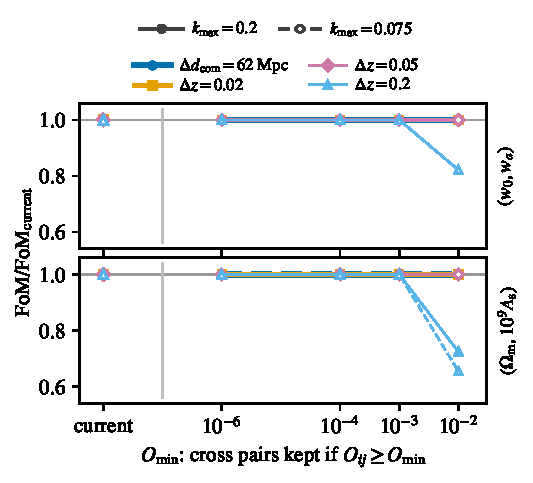
\includegraphics[width=3.5in]{plots/pair_threshold/pair_threshold.pdf}
  \caption{The figures of merit of the fit of
    Section~\ref{sec:threshold} with only the cross pairs whose
    blurred overlap at the default dispersions reaches
    $O_{\min}$, over ${\rm FoM}_{\rm current}$, the figure of merit of
    the current data vector, against $O_{\min}$; ``current'', the
    current data vector with every measured pair, sits left of the
    separator.  Upper
    panel: ${\rm FoM}(w_0, w_a)$; lower: ${\rm FoM}(\Omega_m,
    10^9 A_s)$; the panels share the $y$ axis.  Color, line width and
    marker: the layout; solid, filled markers: $k_{\rm max} =
    0.2\,h$/Mpc; dashed, open: $0.075$; gray: one.  $k_{\rm max}$
    quoted at $z = 0$; each bin is cut at
    $k_{\rm max}/D(\bar{z}_i)$.}
  \label{fig:threshold}
\end{figure}

\section{What would pairs beyond the list add?}
\label{sec:axes}

\paragraph{The question, reversed.}
Section~\ref{sec:threshold} removed pairs from the current list and
found that no listed low-overlap pair carries much.  This section asks
the opposite question: how much would the data vector gain if it
measured pairs \emph{beyond} the current list?  Two families of pair
lists answer it; each contains the current list and grows along one
axis.

\paragraph{The gap axis.}
The first family loosens the first step of the pair rule
(Section~\ref{sec:rule}).  For a whole number $g$ it measures, besides
the current list, every pair of bins whose raw $n(z)$ ranges are at
most $g$ bin widths apart; $g$ counts the gap between the two ranges
in units of the layout's bin width, so $g = 0$ is the current list and
each step in $g$ adds the next chain of pairs, $C^{i,i+2}_\ell$ at
$g = 1$, $C^{i,i+3}_\ell$ at $g = 2$, and so on, with the matching
pairs across the sample boundaries.  On \dcom{} the list grows from
$107$ pairs to $190$, $285$ and $378$ at $g = 1$, $2$ and $3$; the
other layouts grow in the same way.

\paragraph{The $\sv$ axis.}
The second family loosens the second step.  It reruns the
blurred-overlap criterion, $O_{ij} \ge 10^{-6}$
(Eq.~\eqref{eq:overlap}), with every velocity dispersion set to one
common value $s$ in place of the seven defaults.  The dispersion $s$
only \emph{selects} the pairs: the model and the covariance of every
forecast keep the fiducial $\sv$, so this axis measures what a longer
list is worth, not what a stronger blur does.  The lists change late:
on \dcom{} no pair is added until $s = 750$~km/s, where the bins two
apart begin to overlap ($199$ pairs); on $\Delta z = 0.02$ the list
grows at every step, from $147$ pairs at $s = 450$ to $344$ at
$1200$; on $\Delta z = 0.05$ the first new pairs appear only at
$s = 1200$, and on $\Delta z = 0.2$ none ever do.  Among these lists
are the ones that building the pair rule at the edge of the $\sv$
prior would produce (Section~\ref{sec:open}).

\paragraph{How it was computed.}
For each layout the derivative base -- the change of every band of
every spectrum per unit change of every model parameter, the input of
a Fisher matrix -- was computed once, on the layout's largest list
(the union of every point's pairs: $378$, $370$, $178$ and $32$ cross
pairs).  Each point of Figures~\ref{fig:axesgap}
and~\ref{fig:axessigv} is then a row selection: it keeps the rows of
the data vector that belong to its own list (every auto band and the
bands of the list's cross pairs that pass the scale cut; the shear
rows are masked in these forecasts) together with the matching rows and
columns of the covariance, and builds its Fisher matrix from those
alone.  For a Gaussian likelihood this is exact, not an
approximation: selecting the rows equals rebuilding the data set on
the smaller list.  Two checks confirm the machinery: on the shared
rows every derivative base equals the current caches bit for bit, and
the $s = 600$ point of $\Delta z = 0.02$ reproduces, to every digit,
a separate forecast whose data vector, covariance and derivatives
were built on exactly those pairs.

The model is the paper model (Section~\ref{sec:fiducial}): model B +
tilts with $\alpha_2$ fixed at zero in every bin and every $\sv$
prior width six times the exploration width, on the pessimistic
linear-bias prior.  Each list is forecast twice: once with the seven
$\sv$ fitted -- left free, so the quoted errors carry their
uncertainty -- and once with them held at the fiducial values.  The
reference model of Figure~\ref{fig:threshold} behaves similarly; its
grids are in the two figure folders' \texttt{data.json}.

\begin{figure}[tbp]
  \centering
  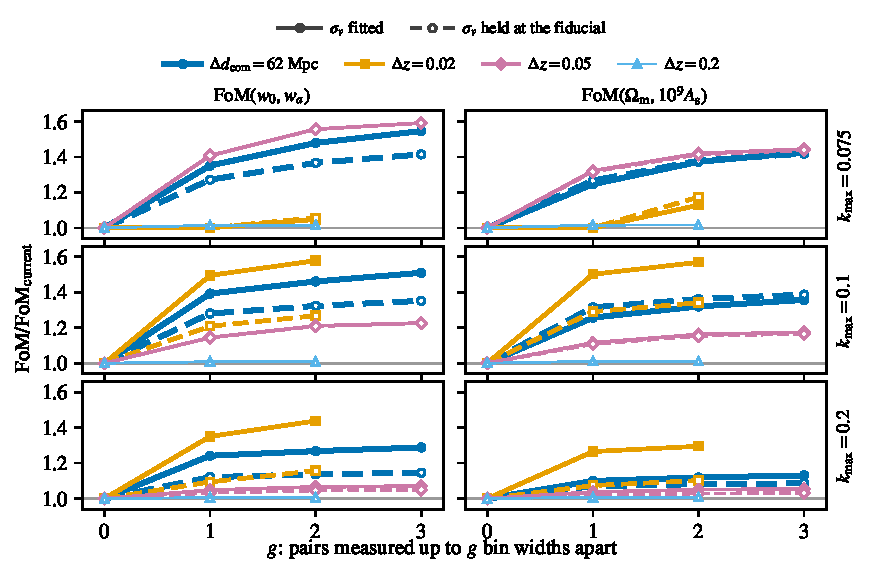
\includegraphics[width=\linewidth]{plots/pair_axes_gap/pair_axes_gap.pdf}
  \caption{The figures of merit of the paper model when, besides the
    current list, every pair whose raw $n(z)$ ranges are at most $g$
    bin widths apart is measured, over ${\rm FoM}_{\rm current}$
    ($g = 0$, the current list).  Rows: $k_{\rm max} = 0.075$, $0.1$
    and $0.2\,h$/Mpc; left column ${\rm FoM}(w_0, w_a)$, right
    ${\rm FoM}(\Omega_m, 10^9 A_s)$; every panel shares one $y$
    range.  Color, line width and marker: the layout; solid lines,
    filled markers: $\sv$ fitted; dashed, open: $\sv$ held at the
    fiducial; gray: one.  $k_{\rm max}$ quoted at $z = 0$; each bin
    is cut at $k_{\rm max}/D(\bar{z}_i)$.}
  \label{fig:axesgap}
\end{figure}

\begin{figure}[tbp]
  \centering
  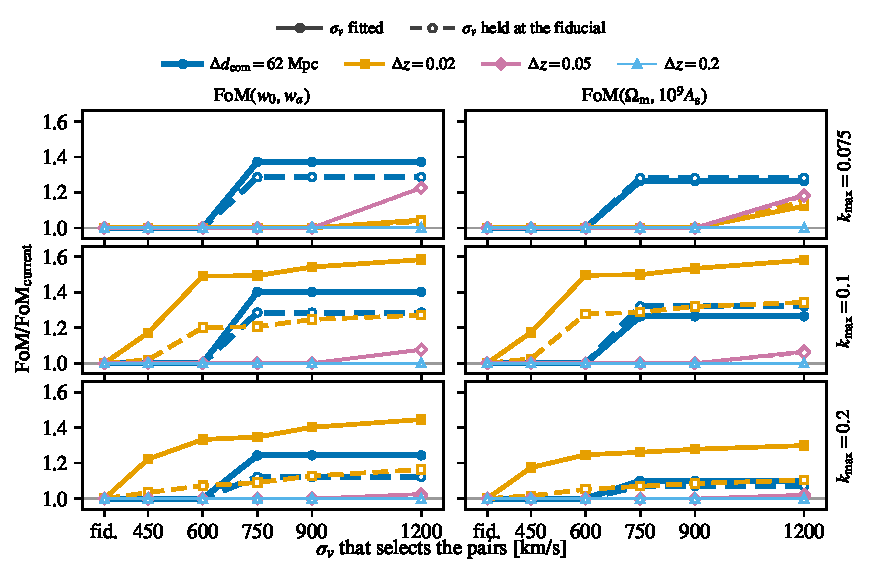
\includegraphics[width=\linewidth]{plots/pair_axes_sigv/pair_axes_sigv.pdf}
  \caption{The figures of merit of the paper model when the pair list
    is selected with every velocity dispersion set to the common
    value on the horizontal axis, over ${\rm FoM}_{\rm current}$
    (``fid.'', the selection at the default dispersions, is the
    current list).  The dispersion only selects the pairs; the model
    keeps the fiducial $\sv$.  Rows: $k_{\rm max} = 0.075$, $0.1$ and
    $0.2\,h$/Mpc; left column ${\rm FoM}(w_0, w_a)$, right
    ${\rm FoM}(\Omega_m, 10^9 A_s)$; every panel shares one $y$
    range.  Color, line width and marker: the layout; solid lines,
    filled markers: $\sv$ fitted; dashed, open: $\sv$ held at the
    fiducial; gray: one.  $k_{\rm max}$ quoted at $z = 0$; each bin
    is cut at $k_{\rm max}/D(\bar{z}_i)$.}
  \label{fig:axessigv}
\end{figure}

\paragraph{What the figures show.}
No ratio can fall below one: the larger list contains the current
one, and giving a Fisher forecast more data can only add information,
never remove it.  The question is how much is added.  On the three
thinner layouts the gain is large -- at its largest point each layout
gains $55$--$59\%$ of ${\rm FoM}(w_0, w_a)$ -- and the first added
chain of pairs carries most of it.  On $\Delta z = 0.2$ the gain
never exceeds $2\%$.  Two kinds of flat stretch in the figures mean
selection, not physics: on the $\sv$ axis a ratio of one before the
first jump only says that the list has not changed yet, and at
$k_{\rm max} = 0.075\,h$/Mpc on $\Delta z = 0.02$ the scale cut
removes every band of the added pairs up to $s = 900$~km/s (and at
$g = 1$), so those points sit at one by the cut.

\paragraph{Why the figures of merit rise.}
The solid and the dashed curves separate two cases: the dashed
curves hold the seven dispersions at their fiducial values, the
solid curves fit them, and on the two thin layouts the solid curves
gain visibly more.  Section~\ref{sec:bias} traces both gains to one
source.  The auto and cross spectra of narrow bins together recover
the three-dimensional clustering information, redshift-space
distortions included~\cite{Asorey2012}; in this model that
information pays off mainly by separating each group's free bias
level and slope from the growth history, and the dispersions ride
on the same separation.

\section{Why the added pairs help: the free bias levels and slopes}
\label{sec:bias}

\paragraph{The question.}
The gains of Section~\ref{sec:axes} call for an explanation.  The
added pairs raise ${\rm FoM}(w_0, w_a)$ by up to $55$--$59\%$ on the
three thinner layouts, and on the two thin layouts they raise it
more when the dispersions $\sv$ are fitted than when they are held
fixed -- although the added spectra barely respond to $\sv$ at all
(Table~\ref{tab:svresponse}).  Which parameters turn the extra
spectra into so much dark-energy precision?  This section answers in
two steps: it first measures how $\sv$ changes each kind of spectrum
and which other parameters change it the same way, then refits every
pair list with blocks of parameters held fixed and reads off which
block the gain flows through.

\paragraph{Cosmology and nuisance parameters.}
The model's parameters are of two kinds.  The cosmological
parameters -- $A_s$, $n_s$, $H_0$, $\Omega_b$, $\Omega_m$, $w_0$ and
$w_a$ -- are the goal.  The rest are nuisance parameters: parameters
that describe the galaxies rather than the universe, but that the
fit must determine from the same data.  In the paper model they are
the linear bias $b_{1,i}$ of every bin, fitted through its
amplitude $\beta_i = b_{1,i}\,D(\bar{z}_i)$ -- the bias times the
growth factor, constant in redshift for a population that is
conserved -- under the pessimistic prior of
Section~\ref{sec:fiducial}: within each sample group the amplitudes
may take any overall level and any slope in redshift without
penalty, while each bin's departure from that straight line, its
residual, carries a Gaussian prior of width $3\%$ of the group's
fiducial amplitude, correlated between bins as
$\exp(-|z_i - z_j|/L)$ with $L = 0.05$.  Per sample come the
higher-order biases $b_2$ and $b_{s^2}$, the counterterm $\alpha_0$,
their redshift tilts, and two shot-noise amplitudes; and there are
the seven $\sv$.  Every figure of merit of Section~\ref{sec:axes} is
marginalized: it quotes the dark-energy errors with every one of
these left free, so that their uncertainty is included in the error
bars.

\paragraph{Templates, and what a degeneracy is.}
For a parameter $p$, its template (or response vector) is the
derivative of every kept band of the data vector with respect to
$p$, each divided by that band's error bar, the square root of that
band's covariance diagonal:
$\sigma_\ell^{-1}\,\partial C_\ell/\partial p$.  The template is the
pattern the parameter imprints on the data, in units of what the
data can resolve, and a fit can tell two parameters apart only as
far as their patterns differ.  Treating each template as an arrow in
a space with one axis per band, the squared length of the arrow is
the information the bands carry on that parameter alone, and the
cosine of the angle between two arrows says how alike two parameters
act: $\pm 1$ is the same pattern up to sign, $0$ is two independent
patterns.  Two parameters whose templates are nearly parallel are
degenerate: they change the predicted spectra in nearly the same
pattern, so the fit measures only a combination of them and both
error bars grow.

\paragraph{How each kind of spectrum responds to $\sv$.}
Table~\ref{tab:svresponse} measures these quantities for $\sv$ and
the spectra of $\Delta z = 0.02$, kind by kind.

\begin{table}[ht]
  \centering
  \small
  \setlength{\tabcolsep}{4.5pt}
  \begin{tabular}{lccccc}
    \hline
    spectra & bands kept & median $d\ln C_\ell/d\ln \sv$
      & information on $\sv$ & $\cos(\sv, b_1)$ & $\cos(\sv, w_0)$ \\
    \hline
    autos $C^{ii}_\ell$ & $1910$ & $-0.086$ & $3.6 \times 10^3$
      & $-0.991$ & $+0.981$ \\
    neighbours $C^{i,i+1}_\ell$ & $1514$ & $+0.293$ & $1.3 \times 10^3$
      & $+0.932$ & $+0.271$ \\
    two apart $C^{i,i+2}_\ell$ & $416$ & $-0.042$ & $1.2$
      & $-0.118$ & $+0.649$ \\
    three apart $C^{i,i+3}_\ell$ & $523$ & $-0.002$ & $0.13$
      & $-0.271$ & $+0.087$ \\
    \hline
  \end{tabular}
  \caption{How the within-sample spectra of $\Delta z = 0.02$ (both
    bins from one galaxy sample) respond to $\sv$ at
    $k_{\rm max} = 0.1\,h$/Mpc (quoted at $z = 0$; each bin cut at
    $k_{\rm max}/D(\bar{z}_i)$), measured on the layout's largest
    derivative base with the diagonal of the covariance, moving every
    dispersion together.  ``Information'': the squared length of the
    response vector defined in the text, the derivative of every kept
    band over its error bar; $\cos$: the cosine between the $\sv$
    response and the named parameter's.  The neighbours are in the
    current list; the pairs two and three apart enter at $g = 1$
    and $2$.}
  \label{tab:svresponse}
\end{table}

Three facts in the table carry the section.
\begin{enumerate}
  \item In the auto spectra, the $\sv$ template is almost exactly
    minus the bias template and almost exactly the $w_0$ template
    (cosines $-0.991$ and $+0.981$): blurring the kernels lowers
    every auto spectrum the way a lower bias or a changed $w_0$
    does.  Fitting $\sv$ is therefore expensive exactly where the
    bins are thin against the blur (Table~\ref{tab:svcost}): on the
    current list it costs a factor $2.7$ of ${\rm FoM}(w_0, w_a)$ on
    $\Delta z = 0.02$ at $k_{\rm max} = 0.1\,h$/Mpc and $2.1$ on
    \dcom{}, against $1.04$--$1.13$ on $\Delta z = 0.05$ and nothing
    on $\Delta z = 0.2$.
  \item The neighbour cross spectra, already in the current list,
    respond to $\sv$ with the opposite sign to the autos: the blur
    moves galaxies across the shared bin edge and so raises the
    neighbour correlation while it lowers the autos -- a pattern no
    bias change mimics.  On the current list they are what limits
    the degeneracy.
  \item The pairs two and three bins apart barely respond to $\sv$:
    their information on $\sv$ is $1.2$ and $0.13$, against
    $3.6 \times 10^3$ in the autos, with median responses near
    zero.  The added pairs do not measure $\sv$; they measure bias
    and cosmology with negligible $\sv$ dependence.
\end{enumerate}

\begin{table}[ht]
  \centering
  \begin{tabular}{lccc}
    \hline
    layout & $k_{\rm max} = 0.075$ & $0.1$ & $0.2$ \\
    \hline
    \dcom{} & $1.98$ / $1.81$ & $2.12$ / $1.90$ & $1.65$ / $1.47$ \\
    $\Delta z = 0.02$ & $2.22$ / $2.24$ & $2.72$ / $2.19$ & $1.78$ / $1.43$ \\
    $\Delta z = 0.05$ & $1.05$ / $1.05$ & $1.04$ / $1.04$ & $1.13$ / $1.10$ \\
    $\Delta z = 0.2$ & $1.00$ / $1.00$ & $1.00$ / $1.00$ & $1.00$ / $1.00$ \\
    \hline
  \end{tabular}
  \caption{The cost of fitting $\sv$ in the paper model:
    ${\rm FoM}(w_0, w_a)$ with $\sv$ fixed over the same figure of
    merit with $\sv$ fitted, on the current list / on the largest
    list of the gap axis.  $k_{\rm max}$ in $h$/Mpc, quoted at
    $z = 0$; each bin is cut at $k_{\rm max}/D(\bar{z}_i)$.}
  \label{tab:svcost}
\end{table}

Table~\ref{tab:svcost} reads the same facts from the side of the
added pairs: they lower the cost of fitting $\sv$ on the two thin
layouts and leave it unchanged where it was already small.

\paragraph{The $\sv$ template, band by band.}
Figure~\ref{fig:svtemplates} draws these facts for one bin.  The
construction is the one of the template figure of
\texttt{notes/fog\us parameter\us degeneracy\us study} (there for
$\alpha_2$ against $\sv$): the $b_1$ and $w_0$ templates of the
bin's sample are scaled by the coefficient that best matches the
$\sv$ template over the kept bands of all $90$ auto spectra, so
every panel shows how far the auto-spectrum match carries over to
the other spectra.  In the auto panel the three curves coincide, and
the leftover after the joint $b_1 + w_0$ match is about a tenth of
an error bar per band: within the autos, $\sv$ is indistinguishable
from a bias change plus a $w_0$ change.  In the neighbour cross the
blur raises the spectrum while the matched bias change lowers it,
and the leftover reaches $1.2$ error bars per band: this is the part
of the $\sv$ pattern that the current list resolves.  In the pair
two apart neither $\sv$ nor the matched bias does much, and the
leftover stays small.  One limitation: the figure moves one $b_1$
per sample, every bin of the sample together, so it cannot show what
the added pairs constrain bin by bin.  That is what the attribution
fits measure.

\begin{figure}[t]
  \centering
  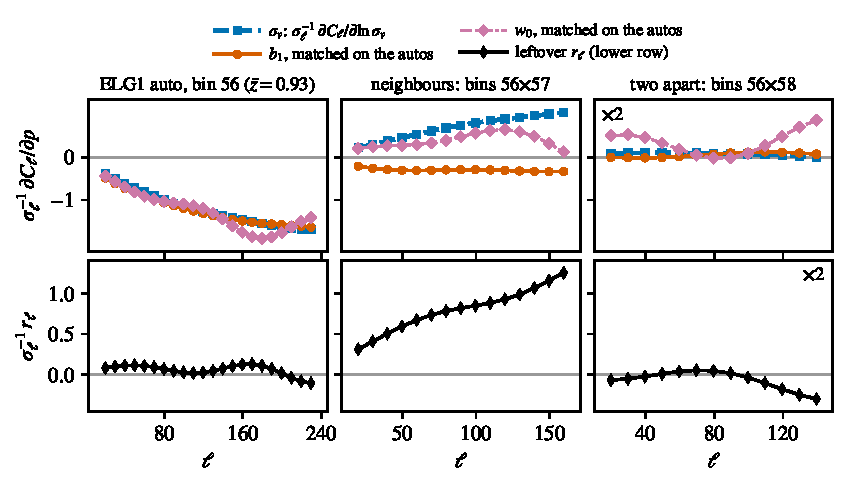
\includegraphics[width=\linewidth]{plots/sv_templates/sv_templates.pdf}
  \caption{The $\sv$, $b_1$ and $w_0$ templates of three
    $\Delta z = 0.02$ spectra of ELG1 bin $56$ ($\bar{z} = 0.93$) at
    $k_{\rm max} = 0.1\,h$/Mpc: the bin's auto spectrum, its cross
    spectrum with the next bin (in the current list) and with the
    bin two apart (added at $g = 1$; drawn at twice its size).  Top
    row: the templates
    $\sigma_\ell^{-1}\,\partial C_\ell/\partial p$, with the $b_1$
    and $w_0$ templates scaled by the coefficient that best matches
    the $\sv$ template over the kept bands of all $90$ auto
    spectra.  Bottom row: the leftover of the joint $b_1 + w_0$
    match, with the same coefficients in every column.
    $k_{\rm max}$ quoted at $z = 0$; each bin is cut at
    $k_{\rm max}/D(\bar{z}_i)$.}
  \label{fig:svtemplates}
\end{figure}

\paragraph{The attribution fits.}
Which parameters turn the added spectra into dark-energy precision?
The test repeats the forecasts of the gap axis with one block of
nuisance parameters held at its fiducial values, as if those
parameters were known exactly.  In a Fisher forecast this takes one
deletion: remove the block's rows and columns from the full Fisher
matrix -- the data term plus every prior, the correlated prior of
the bias residuals included -- and invert what remains.  This is
conditioning, and for a Gaussian likelihood it is exact; it is the
mirror image of marginalizing, which inverts the full matrix first
and then reads off a sub-block, keeping the deleted parameters'
uncertainty in the error bars.  The blocks are the ones of the
nuisance list above: the linear biases $b_1$, held fixed as a whole
(every group's level, slope and residuals together); $b_2$ and
$b_{s^2}$ with their tilts; $\alpha_0$ with its tilt; the shot-noise
amplitudes; and every nuisance parameter at once, with cosmology and
$\sv$ staying free.  The linear-bias block is also split in two.
Per group, the amplitudes $\beta_i$ of its bins are written as a
straight line in redshift plus residuals: the line spans the two
directions the
prior leaves free, the level and the slope, and the residuals span
the directions it charges.  Each part is then held fixed with the
other left free.  Three checks anchor the machinery: with no block
deleted the ratios equal those of Section~\ref{sec:axes} to every
printed digit, deleting the $\sv$ block reproduces the $\sv$-fixed
variants, and with both parts of the split left free the figures of
merit equal the every-parameter-free ones, so the change of basis
loses nothing.

\paragraph{What the fits show.}
Figure~\ref{fig:attribution} draws the gap axis again, block by
block, and Table~\ref{tab:attribution} collects the key numbers.
With every nuisance parameter fixed the gain nearly vanishes: the
largest list is worth $2$--$8\%$ where it was worth $55$--$59\%$,
and the $\sv$-fixed gains collapse the same way, to $2$--$7\%$.  The
line-of-sight clustering information that the added spectra carry by
themselves is therefore worth a few percent once the biases are
known.  Most of the gain enters through the linear-bias block alone:
holding it fixed cuts $\times 1.59$ to $\times 1.07$ on
$\Delta z = 0.05$, $\times 1.58$ to $\times 1.15$ on
$\Delta z = 0.02$ and $\times 1.55$ to $\times 1.26$ on \dcom{}
(each at the scale cut of Table~\ref{tab:attribution}).  Holding
$b_2$ and $b_{s^2}$ fixed removes a smaller part, and the
counterterm and the shot noise change little.  The split of the
linear-bias block decides the reading (Table~\ref{tab:b1split}):
holding only the residuals fixed, with every level and slope still
free, barely changes the gain, while holding only the levels and
slopes fixed removes almost exactly as much as fixing the whole
block.  The gain is carried by the free level and slope of each
group's bias amplitude, not by the correlated per-bin residuals.

\begin{figure}[tbp]
  \centering
  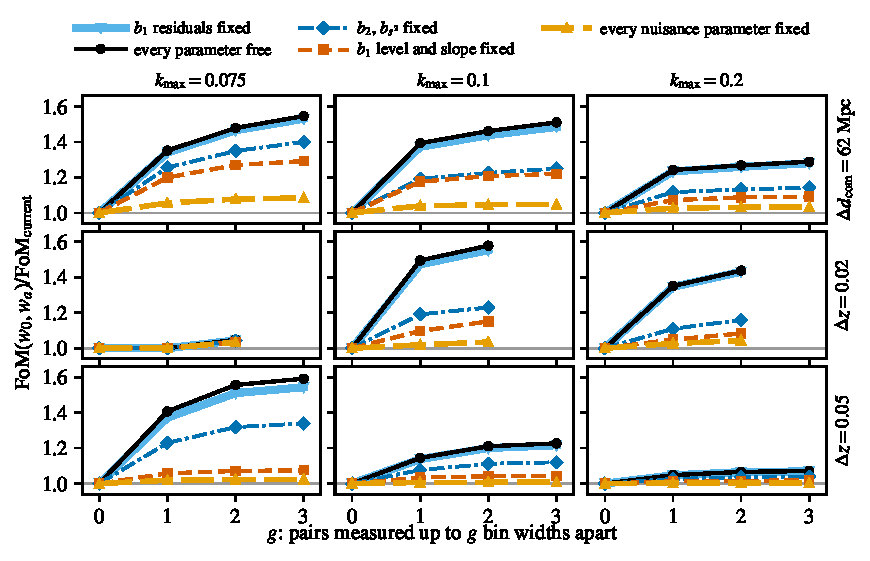
\includegraphics[width=\linewidth]{plots/pair_axes_attribution/pair_axes_attribution.pdf}
  \caption{${\rm FoM}(w_0, w_a)$ of the gap axis over the same
    figure of merit of the current list, with $\sv$ fitted and with
    blocks of nuisance parameters held at their fiducial values by
    conditioning; each curve holds the same block fixed on both
    lists.  Rows: \dcom{}, $\Delta z = 0.02$ and $\Delta z = 0.05$
    ($\Delta z = 0.2$ gains at most $2\%$ and is not drawn);
    columns: $k_{\rm max} = 0.075$, $0.1$ and $0.2\,h$/Mpc, quoted
    at $z = 0$; each bin is cut at $k_{\rm max}/D(\bar{z}_i)$.
    Black solid: every parameter free; sky-blue wide solid
    (triangles), drawn under the black curve: the $b_1$ residuals
    fixed; blue dash-dotted: $b_2$ and $b_{s^2}$ fixed; vermillion
    dashed (squares): the $b_1$ levels and slopes fixed; orange
    long-dashed: every nuisance parameter fixed.}
  \label{fig:attribution}
\end{figure}

\begin{table}[ht]
  \centering
  \small
  \setlength{\tabcolsep}{5pt}
  \begin{tabular}{lccc}
    \hline
    & \dcom{} & $\Delta z = 0.02$ & $\Delta z = 0.05$ \\
    block held fixed & $k_{\rm max} = 0.075$ & $k_{\rm max} = 0.1$
      & $k_{\rm max} = 0.075$ \\
    \hline
    none & $1.546$ / $1.426$ & $1.578$ / $1.569$ & $1.591$ / $1.444$ \\
    all $b_1$ & $1.256$ / $1.312$ & $1.146$ / $1.189$ & $1.072$ / $1.083$ \\
    $b_2$, $b_{s^2}$ & $1.399$ / $1.328$ & $1.230$ / $1.247$ & $1.339$ / $1.230$ \\
    $\alpha_0$ & $1.525$ / $1.392$ & $1.445$ / $1.435$ & $1.464$ / $1.355$ \\
    shot noise & $1.458$ / $1.348$ & $1.459$ / $1.432$ & $1.563$ / $1.417$ \\
    every nuisance & $1.084$ / $1.132$ & $1.035$ / $1.037$ & $1.024$ / $1.031$ \\
    \hline
  \end{tabular}
  \caption{The gain of the gap axis' largest list over the current
    list with one block of nuisance parameters held fixed on both,
    ${\rm FoM}(w_0, w_a)$ / ${\rm FoM}(\Omega_m, 10^9 A_s)$, with
    $\sv$ fitted.  Each layout is quoted at the scale cut where its
    gain is largest ($k_{\rm max}$ in $h$/Mpc, quoted at $z = 0$;
    each bin cut at $k_{\rm max}/D(\bar{z}_i)$) and at its largest
    gap point: $g = 3$, or $g = 2$ on $\Delta z = 0.02$.}
  \label{tab:attribution}
\end{table}

\begin{table}[ht]
  \centering
  \small
  \setlength{\tabcolsep}{5pt}
  \begin{tabular}{lcccc}
    \hline
    layout, $k_{\rm max}$ & all free & residuals fixed
      & level, slope fixed & all $b_1$ fixed \\
    \hline
    $\Delta z = 0.02$, $0.1$ & $1.578$ & $1.553$ & $1.151$ & $1.146$ \\
    $\Delta z = 0.02$, $0.2$ & $1.438$ & $1.431$ & $1.083$ & $1.075$ \\
    $\Delta z = 0.05$, $0.075$ & $1.591$ & $1.543$ & $1.075$ & $1.072$ \\
    \dcom{}, $0.075$ & $1.546$ & $1.530$ & $1.292$ & $1.256$ \\
    \dcom{}, $0.1$ & $1.510$ & $1.484$ & $1.219$ & $1.201$ \\
    \dcom{}, $0.2$ & $1.288$ & $1.279$ & $1.092$ & $1.085$ \\
    \hline
  \end{tabular}
  \caption{The split of the linear-bias block: ${\rm FoM}(w_0, w_a)$
    of the gap axis' largest list over the current list, with $\sv$
    fitted and with parts of the block held fixed on both lists.
    ``Residuals fixed'' keeps every group's level and slope free;
    ``level, slope fixed'' keeps the residuals free.  $k_{\rm max}$
    in $h$/Mpc, quoted at $z = 0$; each bin is cut at
    $k_{\rm max}/D(\bar{z}_i)$.}
  \label{tab:b1split}
\end{table}

\paragraph{The mechanism.}
On large scales the galaxy map of bin $i$ is the matter map times
its linear bias $b_i$ (Section~\ref{sec:groups}), and within each
group the amplitude $\beta_i = b_i D(\bar{z}_i)$ is in effect a free
straight line in redshift -- the bias line of this section: the
prior charges only the per-bin departures from that line.  The auto
spectra cannot pin the line down by themselves.  A higher level
raises every auto spectrum of the group through $b_i^2$ the way a
larger clustering amplitude does, so the level is degenerate with
$A_s$ and the growth of structure; a slope in redshift tilts the
group's spectra against each other the way an evolving growth does,
and how growth evolves with redshift is what $w_0$ and $w_a$
control.  And $\sv$, which in the autos acts like a lower bias,
rides on the same degeneracy.  A cross spectrum depends on the
biases differently, as the product $b_i b_j$, and its ratio to the
two auto spectra -- the correlation coefficient
$C^{ij}_\ell/\sqrt{C^{ii}_\ell C^{jj}_\ell}$ of
Section~\ref{sec:overlap} -- does not depend on the linear biases at
all at linear order.  Each added pair is therefore one more
measurement of the clustering shared by two shells that no bias
line can reshape: it separates the bias line from the growth
history.  This is also why the gain collapses when the levels and
slopes are held fixed, and barely moves when only the residuals
are: where the bias line is known, the auto spectra already measure
what the added pairs would add.

\paragraph{Why the gain is larger with $\sv$ fitted.}
The added pairs carry almost no information on $\sv$ itself
(Table~\ref{tab:svresponse}), yet the $\sv$-fitted curves gain more
than the $\sv$-fixed ones.  The reason is that $\sv$ rides on the
degeneracy between the bias line and growth: in the auto spectra it
acts like a lower bias (Figure~\ref{fig:svtemplates}), so whatever
separates the bias line from cosmology also separates $\sv$.  The
attribution fits show the same link from the other side: with the
bias levels and slopes held fixed, the cost of fitting $\sv$ on the
\emph{current} list falls from $2.7$ to $1.9$ on $\Delta z = 0.02$
at $k_{\rm max} = 0.1\,h$/Mpc, while holding only the residuals
fixed leaves it at $2.7$; with the whole bias block fixed it falls
from $2.1$ to $1.5$ on \dcom{}.  The extra gain of the fitted
curves shrinks with the cost.

\subsection{How the gain depends on the linear-bias prior}
\label{sec:priorgain}

The attribution fits all ran under one prior, the paper's
pessimistic one.  A natural worry is that the gain itself is an
artifact of that choice.  Three priors on the amplitudes $\beta_i$
pass the accuracy test of
\texttt{notes/correlated\us bias\us prior\us v2}, which checks that
the error bars a prior produces still cover the true cosmology
across simulated universes:
\begin{itemize}
  \item the baseline prior: per group a free level and a free slope
    in redshift, plus residuals of width $1\%$ of the group's
    fiducial amplitude ($3\%$ for BGS), correlated as
    $\exp(-|z_i - z_j|/L)$ with $L = 0.2$;
  \item the pessimistic prior, the paper's choice: the same
    structure with $3\%$ in every group and $L = 0.05$;
  \item the free prior: every $\beta_i$ free, with no prior at all.
\end{itemize}
A fourth, the growth-tied prior -- one amplitude per group, with no
slope and no residuals -- fails that accuracy test, so it is
excluded and no figure of merit is quoted for it anywhere in this
note.

Figure~\ref{fig:priorgain} repeats the gap axis under each passing
prior, every point over the same prior's fit on the current list,
and Table~\ref{tab:priorgain} gives the ratios at each layout's
best-gaining scale cut.  The three curves nearly coincide: the
gain agrees within a few percent of the ratio across the priors,
in the expected order -- the looser the residual prior, the
slightly larger the gain, because the added pairs have a little
more left to determine.  The absolute figures of merit do differ
(the tighter the prior, the larger the figure of merit on either
list), but the added pairs raise each by about the same factor.
The agreement follows from the attribution: all three priors leave
each group's level and slope of $\beta(z)$ completely free and
differ only in the residual prior, and the residuals play almost
no part in the gain (Table~\ref{tab:b1split}).  What no passing
prior does is constrain the levels and slopes themselves; the only
tested prior without a free slope is the growth-tied one, which
the accuracy test excludes.

\begin{figure}[tbp]
  \centering
  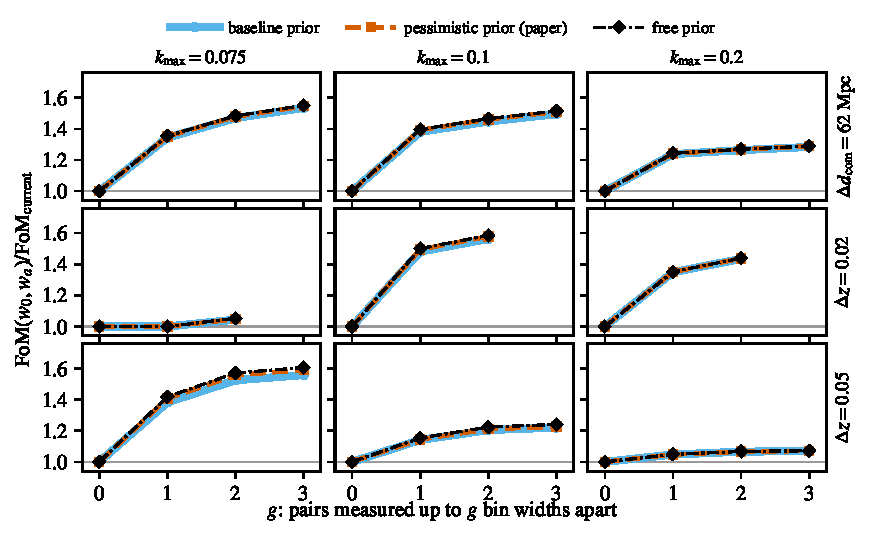
\includegraphics[width=\linewidth]{plots/pair_axes_priors/pair_axes_priors.pdf}
  \caption{${\rm FoM}(w_0, w_a)$ of the gap axis over the same
    figure of merit of the current list, with $\sv$ fitted, under
    each linear-bias prior that passes the accuracy test of
    \texttt{notes/correlated\us bias\us prior\us v2}; each curve is
    normalized to its own prior's fit on the current list.  Rows:
    \dcom{}, $\Delta z = 0.02$ and $\Delta z = 0.05$
    ($\Delta z = 0.2$ gains at most $2\%$ and is not drawn);
    columns: $k_{\rm max} = 0.075$, $0.1$ and $0.2\,h$/Mpc, quoted
    at $z = 0$; each bin is cut at $k_{\rm max}/D(\bar{z}_i)$.
    Sky-blue wide solid (circles): the baseline prior; vermillion
    dashed (squares): the pessimistic prior of the paper; black
    dash-dotted (diamonds): every amplitude free.}
  \label{fig:priorgain}
\end{figure}

\begin{table}[ht]
  \centering
  \small
  \setlength{\tabcolsep}{5pt}
  \begin{tabular}{lccc}
    \hline
    & \dcom{} & $\Delta z = 0.02$ & $\Delta z = 0.05$ \\
    prior & $k_{\rm max} = 0.075$ & $k_{\rm max} = 0.1$
      & $k_{\rm max} = 0.075$ \\
    \hline
    baseline & $1.535$ / $1.422$ & $1.563$ / $1.554$ & $1.558$ / $1.418$ \\
    pessimistic (paper) & $1.546$ / $1.426$ & $1.578$ / $1.569$ & $1.591$ / $1.444$ \\
    free & $1.551$ / $1.430$ & $1.585$ / $1.576$ & $1.606$ / $1.456$ \\
    \hline
  \end{tabular}
  \caption{The gain of the gap axis' largest list over the current
    list under each linear-bias prior that passes the accuracy
    test, ${\rm FoM}(w_0, w_a)$ / ${\rm FoM}(\Omega_m, 10^9 A_s)$,
    with $\sv$ fitted and each ratio taken within one prior.  Each
    layout is quoted at the scale cut where its gain is largest
    ($k_{\rm max}$ in $h$/Mpc, quoted at $z = 0$; each bin cut at
    $k_{\rm max}/D(\bar{z}_i)$) and at its largest gap point:
    $g = 3$, or $g = 2$ on $\Delta z = 0.02$.}
  \label{tab:priorgain}
\end{table}

\paragraph{What this establishes, and what it does not.}
The gain of Section~\ref{sec:axes} is a property of the bias model.
It exists because each group's bias level and slope are completely
free: the added pairs earn their keep by separating that bias line
-- and $\sv$ with it -- from the growth history, while the
correlated residuals play almost no part.  It is not an artifact of
the paper's pessimistic choice: every linear-bias prior that passes
the accuracy test leaves the levels and slopes free and gives the
same gain within a few percent (Section~\ref{sec:priorgain}).  What
remains open is a finite prior on the levels and slopes themselves,
which no passing prior imposes.  A forecast with such prior
knowledge would gain less from the added pairs, with the
level-and-slope-fixed curves of Figure~\ref{fig:attribution} as the
limiting case, but none has been run: how much of the gain such a
prior keeps is an open point (Section~\ref{sec:open}), not a result
of this note.

\section{Open issues}
\label{sec:open}

\begin{itemize}
  \item \textbf{The BGS--LRG1 boundary pair of \dcom{}.}  It is
    measured, as the DESI forecast measures it, although its ranges are
    $0.010$ apart and its blurred kernels barely overlap
    ($3 \times 10^{-7}$, below the second step's threshold); its signal
    is the low-$\ell$ non-Limber correlation alone.
  \item \textbf{The list does not follow $\sv$.}  It is built at the
    default dispersions.  A sampled $\sv$ changes every kernel overlap
    but not which pairs are measured.  Within two prior widths of the
    defaults no unmeasured pair of any layout reaches an overlap of
    $10^{-4}$; what the lists selected at larger dispersions would
    measure is forecast on the $\sv$ axis of Section~\ref{sec:axes}.
  \item \textbf{The pair list at the $\sv$ prior edge.}  Just beyond
    those two prior widths the thin layouts' bins two apart begin to
    overlap by more than $10^{-6}$
    (\texttt{notes/fog\us parameter\us degeneracy\us study}, on the
    pair rule at the edges of the $\sv$ prior).  Those lists have now
    been forecast (Section~\ref{sec:axes}, the $\sv$ axis), and the
    gain is attributed to the free level and slope of each group's
    bias amplitude (Section~\ref{sec:bias}).  What remains open: the
    archiving of
    the largest lists' derivative bases, and the choice of a pair
    list for the paper, which is the authors' and is not made in
    this note.
  \item \textbf{The gain under a prior on the bias levels and
    slopes.}  Every linear-bias prior that passes the accuracy test
    leaves each group's level and slope free, and all of them give
    the same gain within a few percent
    (Section~\ref{sec:priorgain}); with the levels and slopes
    exactly fixed the gain falls from $55$--$59\%$ to $8$--$29\%$
    (Section~\ref{sec:bias}).  A finite prior on them would land
    between those curves; no forecast with one has been run, so
    where the gain lands is not known.
\end{itemize}

\paragraph{Reproducing the figures.}
\texttt{plots/make\us cross\us correlations\us data.py} reads the
project's \texttt{data/} and \texttt{likelihood/} files and writes the
\texttt{data.json} of the first three figure folders, with every
number quoted for them here;
\texttt{plots/pair\us threshold/data.json} is written by the Fisher
notebook \texttt{EXAMPLE\us EVALUATE\us FISHER\us MODEL.ipynb}
(section 11, item 7).  \texttt{plots/make\us pair\us axes\us data.py}
writes the \texttt{data.json} of \texttt{plots/pair\us axes\us gap}
and \texttt{plots/pair\us axes\us sigv} from the pair-axes study's
results file; they hold the full grids of Section~\ref{sec:axes},
for the paper and the reference model both.
\texttt{plots/make\us sv\us templates\us data.py} writes
\texttt{plots/sv\us templates}' \texttt{data.json} from the study's
$\Delta z = 0.02$ derivative base and data set, and
\texttt{plots/make\us pair\us axes\us attribution\us data.py} writes
\texttt{plots/pair\us axes\us attribution}'s from the study's
attribution fits, one file per layout;
\texttt{plots/make\us pair\us axes\us priors\us data.py} writes
\texttt{plots/pair\us axes\us priors}' from the study's prior-gain
fits, one file per layout; these inputs are outputs of the
pair-axes study and sit outside the repository.
Each folder's \texttt{plot\us <name>.py} redraws its figure from that
file alone.

\begin{thebibliography}{99}

\bibitem{Limber1953}
D.~N. Limber,
``The Analysis of Counts of the Extragalactic Nebulae in Terms of a
Fluctuating Density Field'',
ApJ 117, 134 (1953).

\bibitem{Seljak2009}
U. Seljak,
``Extracting primordial non-Gaussianity without cosmic variance'',
Phys. Rev. Lett. 102, 021302 (2009), arXiv:0807.1770.

\bibitem{Jackson1972}
J.~C. Jackson,
``A critique of Rees's theory of primordial gravitational radiation'',
MNRAS 156, 1P (1972).

\bibitem{Kaiser1987}
N. Kaiser,
``Clustering in real space and in redshift space'',
MNRAS 227, 1 (1987).

\bibitem{Asorey2012}
J. Asorey, M. Crocce, E. Gazta\~naga and A. Lewis,
``Recovering 3D clustering information with angular correlations'',
MNRAS 427, 1891 (2012), arXiv:1207.6487.

\bibitem{GrasshornGebhardt2020}
H.~S. Grasshorn Gebhardt and D. Jeong,
``Nonlinear redshift-space distortions in the harmonic-space galaxy
power spectrum'',
Phys. Rev. D 102, 083521 (2020).

\end{thebibliography}

\end{document}
